\documentclass[border=10pt]{standalone}
\usepackage{tikz}
\usetikzlibrary{arrows.meta, positioning, calc}
\usepackage{xcolor}
\usepackage{graphicx}

% Brand colors
\definecolor{Garnet}{HTML}{73000A}
\definecolor{Atlantic}{HTML}{466A9F}
\definecolor{Congaree}{HTML}{1F414D}
\definecolor{Horseshoe}{HTML}{65780B}
\definecolor{Rose}{HTML}{CC2E40}
\definecolor{LightGray}{HTML}{ECECEC}

\begin{document}
\begin{tikzpicture}[
    block/.style={
        draw, thick, minimum width=2.8cm, minimum height=1.2cm,
        align=center, font=\normalsize\bfseries
    },
    data/.style={
        draw, dashed, minimum width=2.4cm, minimum height=1.0cm,
        align=center, font=\normalsize
    },
    arr/.style={-{Stealth[length=3.5mm]}, very thick},
    lbl/.style={font=\small, fill=white, inner sep=2pt},
    imglbl/.style={font=\scriptsize\bfseries, anchor=north, inner sep=2pt},
    every node/.style={font=\normalsize}
]

% =============================================
% PIPELINE ROW
% =============================================

\node[data, fill=Horseshoe!15] (initial) {Initial\\Prompts};
\node[block, fill=Atlantic!12, right=3.0cm of initial] (graph) {Build DSH\\Graph};
\node[block, fill=Congaree!12, right=3.0cm of graph] (qlearn) {Q-Learning};
\node[data, fill=Horseshoe!15, right=3.0cm of qlearn] (optimized) {Optimized\\Prompts};

\draw[arr] (initial.east) -- (graph.west);
\draw[arr] (graph.east) -- (qlearn.west);
\draw[arr] (qlearn.east) -- (optimized.west);

% Q-learning loop
\draw[arr, Rose] (qlearn.south) -- ++(0,-0.6) -| (graph.south);
\node[font=\small\itshape, text=Rose] at ([yshift=-0.8cm]$(graph.south)!0.5!(qlearn.south)$) {$N = 30$ episodes};

% =============================================
% IMAGES ROW (below pipeline)
% =============================================

\node[below=2.0cm of initial, anchor=north] (img_initial) {
    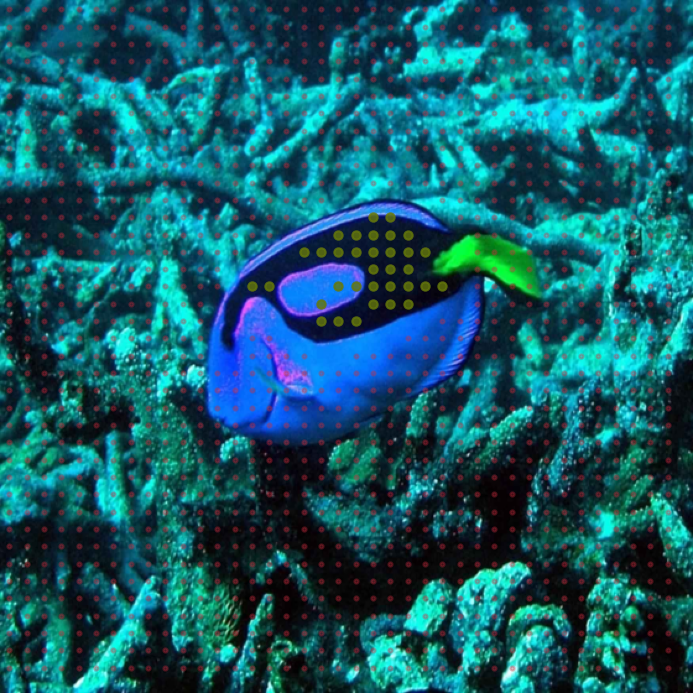
\includegraphics[width=3.8cm]{graph_stage/initial_prompts_clean.png}
};
\node[imglbl] at (img_initial.south) {34 pos, 1413 neg};
\draw[dashed, gray] (initial.south) -- (img_initial.north);

\node[below=2.0cm of graph, anchor=north] (img_graph) {
    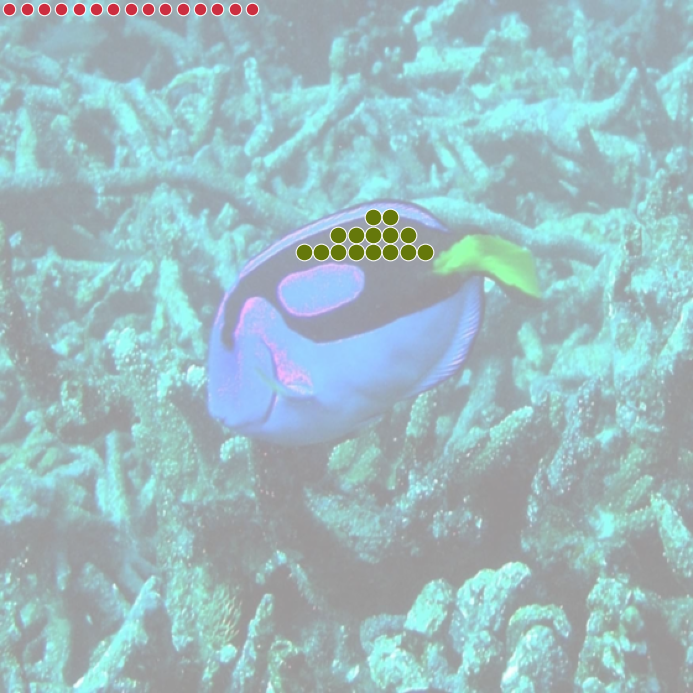
\includegraphics[width=3.8cm]{graph_stage/graph_edges_clean.png}
};
\node[imglbl] at (img_graph.south) {5 edge types, $\sim$2M edges};
\draw[dashed, gray] (graph.south) -- (img_graph.north);

\node[below=2.0cm of qlearn, anchor=north] (img_qlearn) {
    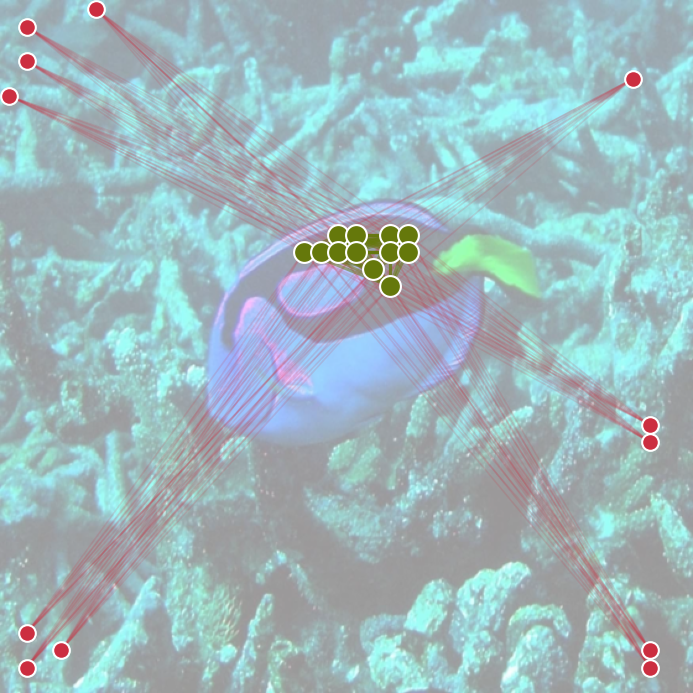
\includegraphics[width=3.8cm]{graph_stage/optimized_graph_clean.png}
};
\node[imglbl] at (img_qlearn.south) {Subset selection};
\draw[dashed, gray] (qlearn.south) -- (img_qlearn.north);

\node[below=2.0cm of optimized, anchor=north] (img_optimized) {
    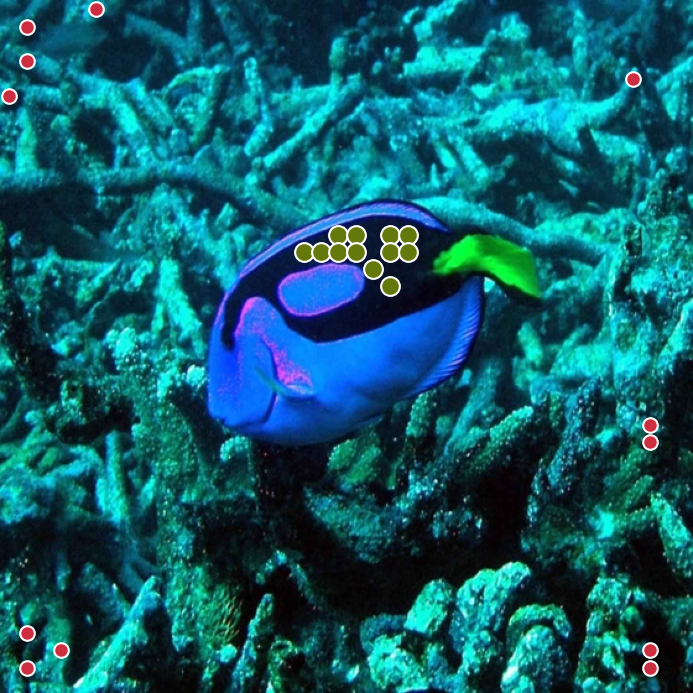
\includegraphics[width=3.8cm]{graph_stage/optimized_prompts_clean.png}
};
\node[imglbl] at (img_optimized.south) {12 pos, 12 neg};
\draw[dashed, gray] (optimized.south) -- (img_optimized.north);

% =============================================
% Edge type legend
% =============================================
\node[anchor=north west, font=\scriptsize] at ([yshift=-0.5cm]img_graph.south west) {
    \begin{tabular}{@{}ll@{}}
    \textcolor{Horseshoe}{\rule{0.5cm}{2pt}} & feature\_pos (pos$\leftrightarrow$pos) \\
    \textcolor{Rose}{\rule{0.5cm}{2pt}} & feature\_cross (pos$\leftrightarrow$neg) \\
    \textcolor{Atlantic}{- - -} & physical\_cross (pos$\leftrightarrow$neg) \\
    \end{tabular}
};

\end{tikzpicture}
\end{document}
